\clearpage
\section{Transport og drivende kraft}\label{sec:transport_effort}
Til nå har vi antatt at vi kjenner transporten mellom hvert system. Hva gjør vi hvis vi ikke kjenner denne transporten? Svaret er kanskje ikke overraskende; Vi modellerer den! Men hvordan modellerer vi transporten ($\hat{\Phi}_{a|c}$, $\hat{\Phi}_{b|c}$, $\dots$) mellom de forskjellige systemene? Spenn setebeltet fast for nå beveger vi oss inn i termodynamikken.

\subsection{Indre energi og effortvariabler}\label{sec:indre_effort} Endringen av en ekstensiv variabel $\hat{\Phi}$ er bestemt av intensive variaber. Vi gidder ikke bruke mye tid på å forklare all matematikken bak drivende kraft (Kapittel 5.1 i ABC-heftet) så vi hopper rett inn i det som kalles \textit{effortvariabler} ($\pi$). Effortvariabler er intensive variabler definert som endringen av indre energi U ved forskjellige kriterier. Indre energi er en funksjon av entropi, volum og stoffmengde (S,V,\underline{\textbf{n}}) som vi finner i ligningen for total energi. I ligningene under ser vi sammenhengen mellom indre energi og effortvariabler.  Notasjonen med underindekser til brøken betyr at de variablene holdes konstant.

\begin{equation}
\label{eq:indre_energi}
\begin{split}
\Big(\frac{\partial U}{\partial S}\Big)_{V,\underline{\textbf{n}}} =:&\hspace{0.1cm} T \\
\Big(\frac{\partial U}{\partial V}\Big)_{S,\underline{\textbf{n}}} =:&\hspace{0.1cm} -p \\
\Big(\frac{\partial U}{\partial \underline{\textbf{n}}}\Big)_{S,V} =:&\hspace{0.1cm} \mu
\end{split}
\end{equation}

Det viktigste å huske fra Ligningene i \ref{eq:indre_energi} er at temperatur, trykk og kjemisk potensial er effortvariablene som sørger for endringer i ekstensive variabler. Med andre ord er det endring i T, p og $\mu$ som sørger for transport fra et system til et annet. For eksempel vil varmetap i en bolig skje fordi temperaturen utenfor er lavere enn temperaturen inne. Det vil si at forskjellen mellom temperaturen ute og inne sørger for transport av varme ut fra boligen. 

\textbf{Ekstra}:\\ 
Konsentrasjon og molbrøk er ikke effortvariabler, men istedet utledet fra kjemisk potensial. Ofte brukes konsentrasjon i uttrykk for transporten i form av diffusjon eller kjemisk reaksjon. Det er ikke nødvendigvis feil å bruke konsentrasjon i beregningene, men ved likevekt vil ikke nødvendigvis konsentrasjonsforskjellen mellom de to stoffmengdene være null, men forskjellen i det kjemiske potensialet vil alltid være null.  

\subsection{Konduksjon VS konveksjon}\label{sec:konveksjon_konduksjon}
Dette er to ord som ofte blir brukt om hverandre i varmetransport og som kan forvirre mange. 

\begin{itemize}
    \item \textbf{Konduksjon}: overføring av varme fra et molekyl til et annet via gnisninger mellom molekylene
    \item \textbf{Konveksjon}: varmeoverføring på grunn av transport av masse med høy indre energi
\end{itemize}
Eksempel på konvenksjon er kulden du merker når du åpner et vindu på en kald vinterdag. Alle de kalde luftmolekylene, med lavere indre energi enn molekylene i rommet, transporteres inn i stuen din og kjøler deg ned. Konduksjon er transporten av varmen gjennom veggen og ut til den kalde luften. Hvorfor er dette viktig å vite, spør du. Jo, for når du skal tegne opp en topologi for varmetransport vil ikke konveksjon behandles likt som konduksjon i en modell. Konveksjon behandles som transport av indre energi (som oftest entalpi). Men ikke tenk for mye på dette. PS: Stråling er også en form for varmetransport som du sikker husker fra Strømningsfaget. 

\subsection{Generell transportlov}
Hvis vi har transport av en ekstensiv variabel fra et system til et annet hvor posisjonen i system er betydelig for transporten ($\hat{\varphi}$), så er det vanlig å sette opp en differensialligning for endringen av effortvariabelen. NB: her bruker vi $\hat{\varphi}$ istedet for $\hat{\Phi}$ siden den ekstensive variabelen er avhengig av posisjon.

\begin{equation}
    \label{eq:transport_lov}
    \hat{\varphi} = -c\frac{\partial \pi}{\partial \underline{\textbf{r}}}
\end{equation}
$c$ er konduktiviteten (utrykk for mostanden) og $\underline{\textbf{r}}$ er retningene som $\hat{\varphi}$ transporteres gjennom. Denne likningen ligner på Ficks lov eller Fouriers lov som du, forhåpentligvis, har sett tidligere i henholdsvis RekTek og Termo GK. Til vår glede er \cref{eq:transport_lov} Ficks og Fouriers lov på generell form. 

\textbf{Eksempel:}\\
Si at vi har en topologi som er representert med to lumped systems med transport mellom de to systemene, se \cref{fig:transport_topologi1}. 

\begin{figure}[H]
    \centering
    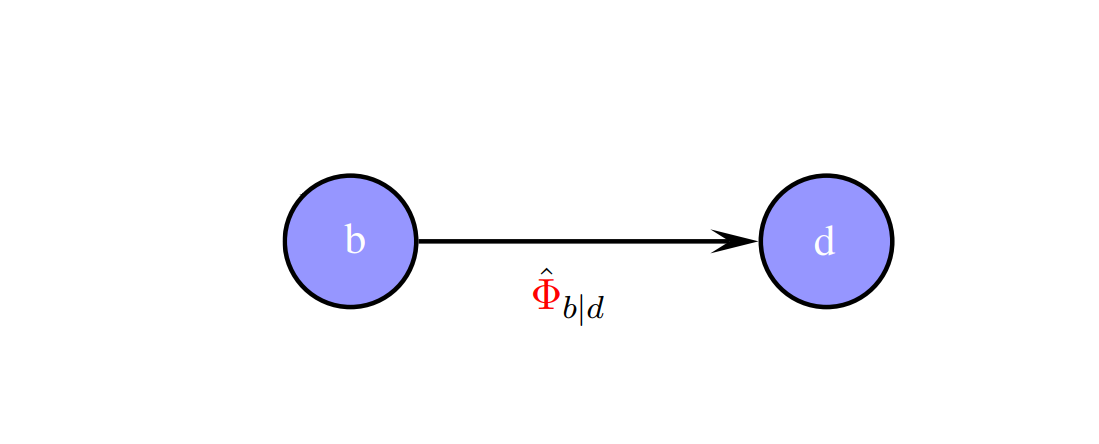
\includegraphics[scale=0.3]{Figures/Transport_topologi.png}
    \caption{Topologi av to lumped systems med transort fra $b$ til $d$.}
    \label{fig:transport_topologi1}
\end{figure}

Bruker vi \cref{eq:transport_lov} for transporten mellom $b$ og $d$ ser vi at transporten, $\hat{\Phi}_{b|d}$, er avhengig av endringen av $\pi$ i system $b$ og $d$: 
\begin{equation}
\hat{\Phi}_{b|d} = \hat{\varphi}_{b|d} = -c_{b|d}\frac{\partial \,( \pi_{b|d})}{\partial \, r_{b|d}}
\end{equation}

\subsection{Lineær modell for transport}\label{sec:linear_transport}
Anta at vi er interessert i en enkel modell for transporten mellom $b$ og $d$, som vist i Figur \ref{fig:transport_topologi1}, og ikke har informasjon om hvordan $\pi$ endrer seg fra $b$ til $d$. Da er det rimelig å benytte seg av en lineær modell for transporten mellom systemene. Vi lineariserer endringen av effortvariablen fra system $b$ til $d$ og får en modell som er grafisk representert i \cref{fig:linearized_transport}. 

\begin{figure}[H]
    \centering
    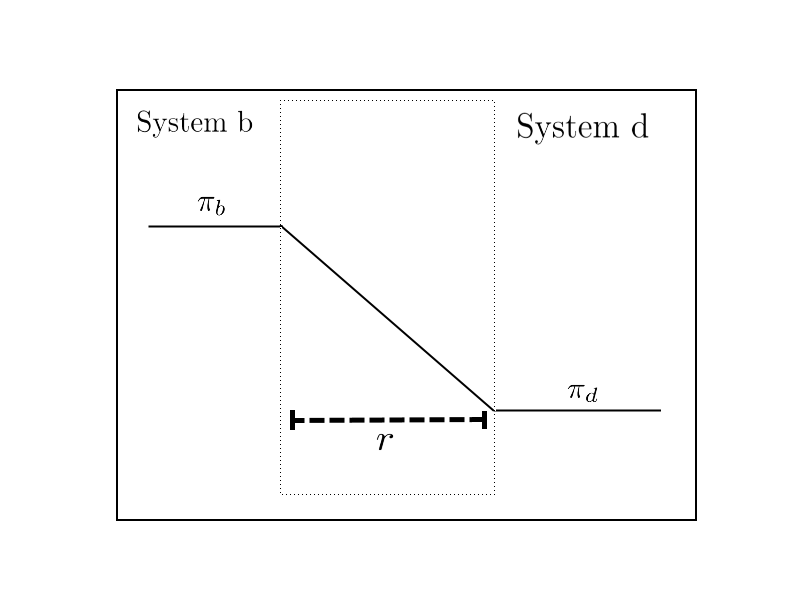
\includegraphics[scale=0.5]{Figures/linearized_transport.png}
    \caption{Grafisk representasjon av lineariseringen av $\frac{\partial \pi}{\partial \underline{\textbf{r}}}$  som viser den lineære endringen i effortvariabelene fra system $b$ til system $d$. $r$ er avstanden mellom systemene. }
    \label{fig:linearized_transport}
\end{figure}
Lineariseringen av $\frac{\partial \pi}{\partial \underline{\textbf{r}}}$ gjøres ved bruk av en Taylor utvidelse av første orden, se \cref{sec:distributed}. Dette gir oss en lineær modell for transporten av den ekstensive variabelen:



\begin{equation}
    \label{eq:transportlov_linear}
    \hat{\Phi}_{b|d} = -k_{b|d}(\pi_b-\pi_d)
\end{equation}

Denne likningen kan vi nå substituere inn i balansene fra  \cref{sec:massetransport}. Merk at vi har en lineær modell som ikke nødvendigvis er korrekt. Hvis transporten mellom to systemer er essensielt for modellen kan det være lurt å benytte seg av andre metoder for modellering av transport f. eks. \cref{eq:transport_lov}, Governing equations (ikke pensum), Navier Stokes (ikke pensum) eller shell balance. 

